\documentclass[conference]{IEEEtran}

\usepackage[latin1]{inputenc}
\usepackage[T1]{fontenc}
\usepackage[norsk, english]{babel}
\usepackage{epsfig, times}
\usepackage{longtable}
\usepackage{fancyhdr}
\usepackage{amsmath}
\usepackage{verbatim}
\usepackage{cite}
\usepackage{textcomp}
\usepackage{graphics}
\usepackage{subfigure}
\usepackage{algorithm}
\usepackage{algorithmic}
\usepackage{wrapfig}
\usepackage{url}
\usepackage{ulem}
\usepackage{color,soul}
\usepackage{graphicx}

\normalem

\newcommand\PH[1]{\textcolor{blue}{(\it #1)}}
\newcommand\HKS[1]{\textcolor{green}{(\it #1)}}

\begin{document}

%\title{Game server architectures for parallel execution and scalability}
\title{A Demonstration Of a Lockless, Relaxed Atomicity State Parallel Game Server (LEARS)}

\author{
  Kjetil Raaen, H{\aa}vard Espeland, H{\aa}kon Kvale Stensland,
  Andreas Petlund, P{\aa}l Halvorsen, Carsten Griwodz\\
  NITH, Norway \ \ \ \ Simula Research Laboratory, Norway \ \ \ \ 
  IFI, University of Oslo, Norway\\
  Email: raakje@nith.no, \{haavares, haakonks, apetlund, paalh, griff\}@ifi.uio.no
}


\date{\today}
\maketitle


\begin{abstract}
Supporting thousands of interacting players in a virtual world poses
huge challenges with respect to processing. To host as many
players as possible, the server software has
to implement support for massive parallelism. Earlier work within the
field suggests that this is difficult due to synchronization issues, but
in this paper, we present the design and implementation of a game server
architecture based on a model that allows for massive parallelism.
%The server design is evaluated using
%replayed traces from actual gameplay to create server traffic. 
%We also discuss challenges that arise as different
%dependency requirements are introduced to the system. 
Our prototype is evaluated using traces from live game sessions where
we measure the server response time for all objects that need timely
updates. We also measure how the response time for the multi-threaded
implementation varies with the number of threads used. Our results
show that the challenge of scaling up a game-server can be an
embarrassingly parallel problem.
\end{abstract}

\section{Introduction}

%Over the last decade, online multi-player gaming has experienced an
%amazing growth. Providers of the popular online games must deliver a
%reliable service to thousands of concurrent players meeting strict
%processing deadlines in order for the players to have an acceptable
%quality of experience (QoE). 

%% Game types and server architectures
%% Game server architecture models.
%% -FPS, RTS and small, local servers with low pings.
%% -Separated gameworld instances, each with < 1000 players
%% -Shards, grids and area of interest.

%% Game designs that allow thousands of players to interact in a small
%% space is also challenging.

One major goal for large game providers is to support as many
concurrent players in a game-world as possible while preserving the
strict latency requirements in order for the players to have an
acceptable quality of experience (QoE). In order to achieve this,
game-worlds are typically partitioned into areas-of-interest to
minimize message passing between players with no interaction and to
allow the game-world to be divided between servers. This approach is
however limited by the distribution of players in the game-world, and
the problem is that the distribution of players is heavy-tailed with
about 30\% of players in 1\% of the game area~\cite{chen-2006}. 

In such scenarios, the important metric for online multi-player games
is latency. Claypool et. al.~\cite{claypool++-2006} classify different
types of games and conclude that for first person shooter (FPS) and
racing games, the threshold for an acceptable latency is 100ms. For
other classes of networked games, like real-time strategy (RTS) and
massively multi-player online games (MMOGs) players will tolerate
somewhat higher delays, but there are still strict latency
requirements in order to provide a good QoE. The accumulated latency
of network transmission, server processing and client processing adds
up to the latencies that the user is experiencing, and reducing any of
these latencies will improve the user's experience.

%There is a prevailing belief in the need for single threaded execution
%of the game event loop in order to preserve what is seen as critical
%dependencies in the game~\cite{Abdelkhalek2004++} \PH{Har vi noen
%  eksempler her som bruker dette??}. Due to this
%constriction, even when provisioning for scalability in designing an
%online game, service providers still find that the processing power on
%the server side is becoming scarce~\cite{Cai2002++}.
%\PH{Kan vi omformulere dette? \cite{Cai2002++} er eldre enn %~\cite{Abdelkhalek2004++}}
The traditional design of massively multi-player game servers rely \textit{sharding} for scalability beyond what a single CPU core can handle. \textit{Sharding} involves making a new copy of an area of a game, where players in different copies are unable to interact. This approach eliminates most requirements for communication between the processes running individual shards. An example of such a design can be found in~\cite{chu-2008}.

The industry is now experimenting with
implementations that allow for a greater level of
parallelization. One known example is Eve Online \cite{drain-2008}. With LEARS, we
take this approach even further and focus on how many players can be
handled in a single segment of the game world. We present a model that
allows for better resource utilization of multi-processor, game server
systems which should not replace spatial partitioning techniques for
work distribution, but rather complement them to improve on their
limitations. Furthermore, a real prototype game is used for evaluation
where captured traces are used to generate server load. We compare
multi-threaded and single-threaded implementations in order to measure
the overhead of parallelizing the implementation and showing the
experienced benefits of parallelization. The change in responsiveness
of different implementations with increased load on the server is
studied, and we discuss generic elements of this game design which
impact of our chosen platform of implementation.

Our results indicate that it is possible to design an ``embarrassingly
parallel'' game server. We also observe that the implementation is
able to handle a quadratic increase of in-server communication when
many players interact in a game-world hotspot.


\section{Design and Implementation}\label{sec:design}

Traditionally, game servers have been implemented much like game
clients. They are based around a main loop, which updates every active
element in the game.  These elements include for example player characters,
non-player characters and projectiles. The simulated world has a list
of all the active elements in the game, and typically calls an
"update" method on each element. In this method, the active element
will perform all its actions for the time-slot. 
Since these are sequential operations all actions can be performed directly. The
character reads input from the network, performs updates on itself
according to the input, and updates other elements with the results of
its actions.

To make a parallel game server with minimal locking, the system needs
to be redesigned from the ground up with parallelism in mind.
\subsection{Parallel main loop}

\begin{figure}
\centering
\vspace{-3mm}
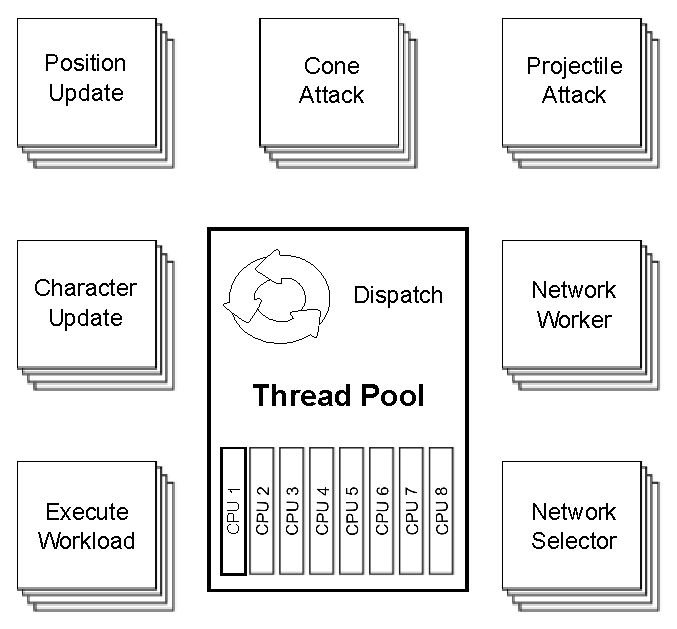
\psfig{file=FIG/server.eps,width=7.5cm}
\vspace{-2.5mm}
\caption{Design of the Game Server}
\vspace{-2.5mm}
\label{fig:server}
\vspace{-2.5mm}
\end{figure}

The system demonstrated here uses a threadpool executor as the core of
the main loop.  When an active element is created in the world, it
is scheduled for execution by the thread pool executor. When it
executes, the active element updates its state exactly as in the
single threaded case. When the task is finished for one time slot, it
can reschedule itself for the next slot, delayed by a specified time.
This allows active elements to have any lifetime from one-shot
executions to the duration of the program. It also allows different
elements to be updated at different rates, depending on the
requirements of the game developer.

The demo setup allows the user to interactively change the number of
threads in the threadpool. By setting the number of threads below the
number of cores it is, by means of the real-time monitoring, possible
to examine how well the cores are utilized.


\subsection{Use of locking}
The thread pool executor used as described above does not constrain
which tasks are executed in parallel. Therefore, all systems elements
must allow any of the other elements to execute concurrently. This
places one simple constraint on what an element can do; i.e., 
\emph{Elements can only update their own state, but read any state.}

This is sufficient because there is no need to establish consistent
ordering of events. This might sound counter intuitive, but it works since
the gameworld already is a simple simulation with a whole series of
approximations. All clients are connected to the server through
individual network links, with vastly different latencies.  The
clients are also run on different computers, with different update
frequencies. If player A performs an action slightly before player B,
this ordering is not necessarily kept by the server in the multi-threaded 
case. Running client update requests in parallel does not
aggravate this problem.

Another potential reason for locking is to keep state changes
atomic. This is also unnecessary due to the nature of the
problem. Consider the following example: Character A moves while
character B attacks. If only the X coordinate of character A is
updated at the point in time when the attack is executed, the attack
will see character A at position $(X_{t+\Delta T},Y_{t})$. This
position is within the accuracy of the simulation which in any case is
no better than the distance an object can move within the timeline $\Delta T$. The
only requirement for this to work is that assignment operations are
atomic.

The end result of our proposed design philosophy is that there is no
synchronization in the server under normal running conditions.

\subsection{Message passing}
Blocking queues~\cite{java:blockingqueue} are queue implementations
that are synchronized separately at each end. This means that elements
can be removed from the queue simultaneously with elements being
added. Each of these operations is also extremely quick, so the
probability of blocking is low.

These are used by the implementation to allow information to be passed
between active objects. Each active object that can be influenced by
others has a blocking queue of messages. During its update, it will
read and process the pending messages from its queue. Other active
elements put messages in the queue to be processed when they need to
change the state of other elements in the game.


\section{Example Game}
 This demonstration uses an implementation of a very simple game which
nonetheless contains all typical elements of a full Massively Multiplayer
Online game, with the exception of persistent state. The game itself
is simple. Each player controls a small circle ("the character") with
an indicator for which direction they are heading. The characters are
moved around by pressing keyboard buttons. They also have two attacks:
One projectile and one instant area of effect attack. Both attacks are
aimed straight ahead. If an attack hits another player character, the
attacker gets a positive point, and the character that was hit gets a
negative point. This simple game provides examples of all the elements
of the design described above:\begin{itemize}
\item The player character is a long lifetime active object. It
  processes messages from clients, updates states and potentially
  produces other active objects (attacks). In addition to position,
  which all objects have, the player also has information about how
  many times it has been hit and how many times it has hit others as
  part of its state. The player character also has a message queue to
  receive messages from other active objects. At the end of its
  update, it will enqueue itself for the next update unless
  the client has disconnected.
\item The frontal attack is a one shot task that finds player
  characters in its designated area and sends messages to those hit so
  they can update their counters, as well as back to the attacking
  player informing about how many were hit.
\item The projectile is a short lifetime object that moves in the
  world, checks if it has hit anything and reschedules itself for
  another update, unless it has hit something or ran to the end of its
  range. The projectile can only hit one target.
\end{itemize}

Our implementation has no spatial partitioning, we are interested in the worst
case, hence the numbers presented in this paper assume all players can see each
other at all times. This means that the number of messages and interactions by
necessity grows by the number of clients squared.

To simulate workload that grow linearly with number of players, especially
collision checks with the ground and other static objects, we have included a
synthetic load. The synthetic load is designed to emulate collision checks with
a grid representing the ground in the virtual world. To achieve this, we have
created an array of floating point values representing a part of the gameworld.
For each scheduled update, each character has to perform a square operation on
a given number of elements in the array. The operation is seeded with a
randomly generated value in order to avoid runtime optimizations in the virtual
machine. Which elements are processed depends on the player's position in the
gameworld. How many array elements are processed determines the severity of the
load. By adding the synthetic load, the cache is dirtied and the game server
processes becomes more realistic compared to a large-scale MMORPG. The demo
setup allows the user to experiment with different levels of synthetic load.

\section{Demonstration}\label{sec:demo}

The demo setup consists of three machines and is illustrated in
figure~\ref{fig:demo-setup}. One machine is the game server. For this
purpose, we are using a four-core CPU, which gives us enough parallel
processing power to illustrate improvements over single threaded
implementations. Another machine plays back a trace of actual gameplay
in as many instances needed to emulate high loads on the server. The
client simulation machine is not a bottleneck, since simulating
clients requires very little calculation. The last machine is for
running the real game client, so the experimenter can see what is
going on on the server and play the actual game.

The demo setup also includes a wireless router and and a web-server
for sharing the game client with interested attendees. This setup
allows others to download the client and play the game during the demo
session.

\begin{figure}
\centering
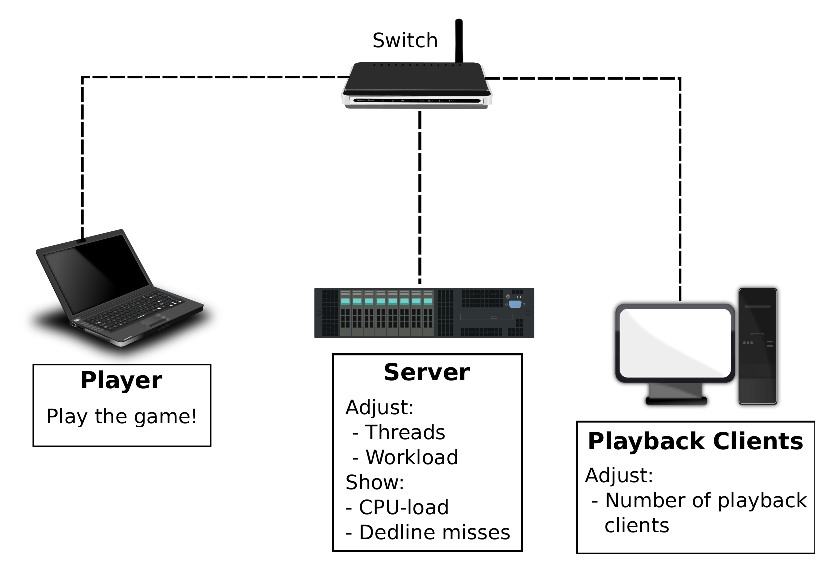
\psfig{file=FIG/demo-setup.eps,width=7cm}
\vspace{-1mm}
\caption{Setup of the demonstration}
\vspace{-2.5mm}
\label{fig:demo-setup}
\vspace{-2.5mm}
\end{figure}

For the purposes of this demonstration, the game server has been
updated with an interactive graphical user interface. Using this
interface, an experimenter can configure the conditions for the
experiment on the fly, while watching the results in real-time.

\begin{figure}
\centering
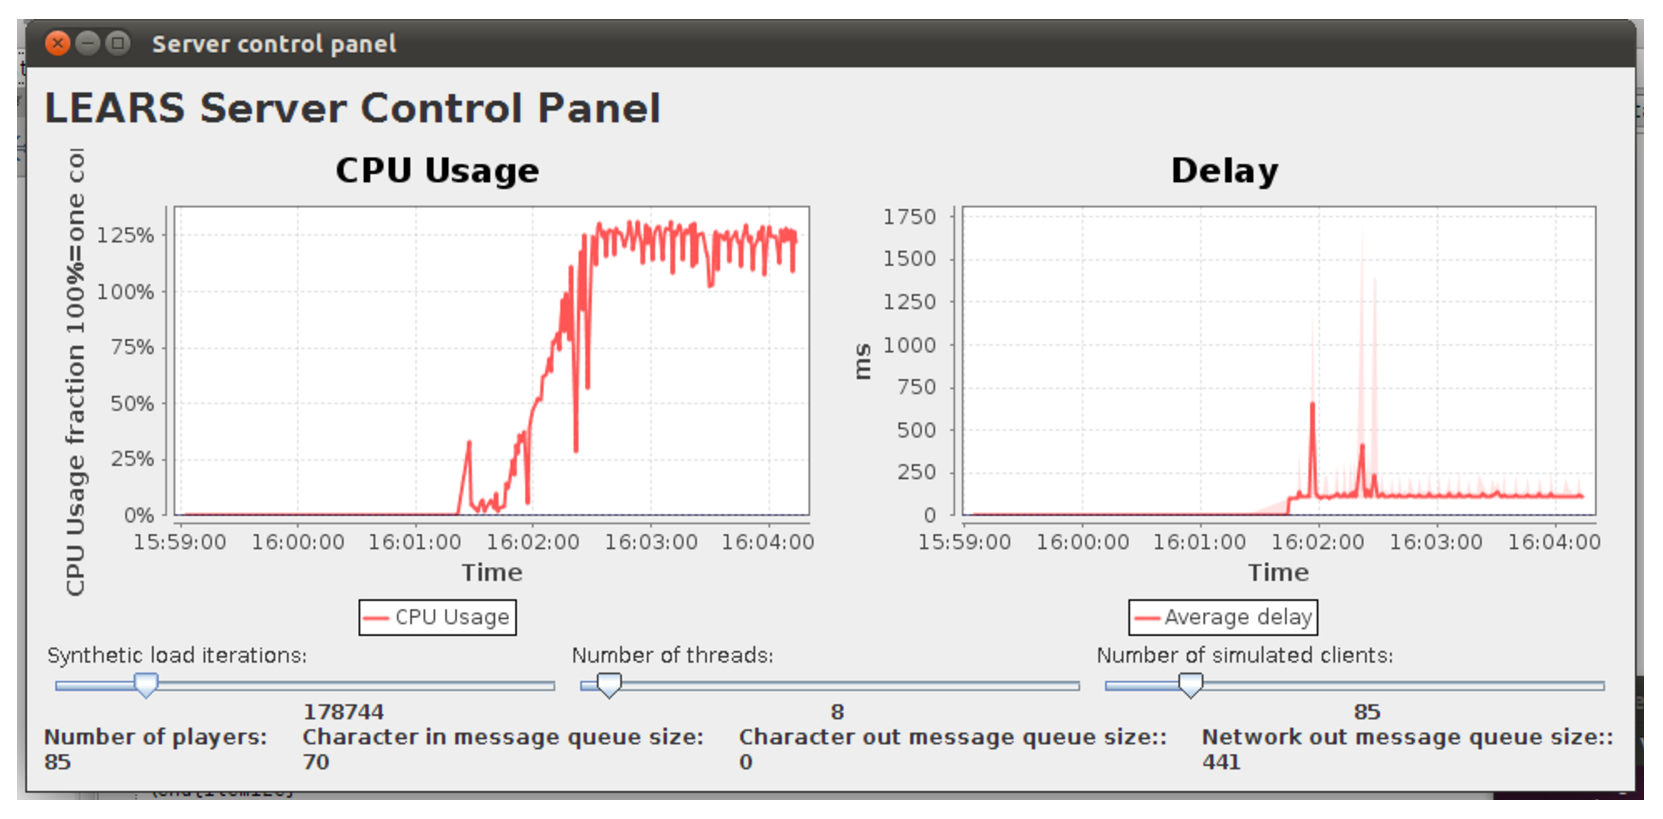
\psfig{file=FIG/gui.eps,width=9cm}
\vspace{-3mm}
\caption{Screenshot of the game server GUI}
\vspace{-2.5mm}
\label{fig:gui}
\vspace{-2.5mm}
\end{figure}

The GUI, shown in figure~\ref{fig:gui} has two plots, both updated
once every second. The left plot shows CPU usage vs. time. The right plot displays the interval between
updates. The system is designed to do an update every 100ms. Increases
above this level is considered deadline misses. The red line shows the
average value for the current measurement interval, the pink outline
shows the highest and lowest values. This is the main performance
metric for the server system, and any value above approximately 250ms
will severely deteriorate the QoE for players of the game.

Below the plots there are three sliders. One controls the number of
iterations for the synthetic load. The experimenter can adjust this to
change the intesnity of the load generated by each player. The next
slider sets the number of threads available to the thread pool. The
final slider instructs the playback client to start or stop playback
instances in order to reach the chosen number.

\section{Conclusion}
Using this setup it is possible to study, in real-time, how our
Lockless, Relaxed Atomicity State Parallel Game Server (LEARS) handles
different conditions, by varying the number of players, the number of threads and the synthetic load associated with each player.
The demo allows us to thoroughly investigate how the system reacts when the described parameters are changed.

Using this demonstration we can see clear indications that, if designed from the ground up with
parallelism in mind, game servers can scale well with the number of
cores on a unified memory multiprocessor system, even in the case
where all players must be aware of all other players and their
actions.


\section*{Acknowledgements}
\noindent
This work has been performed in the context of the  \textit{iAD} centre for
Research-based Innovation (project number 174867) funded by the
Norwegian Research Council.
%% Kjetil: Insert NITH in acknowledgements if needed.

\bibliographystyle{abbrv}
\bibliography{all}

\end{document}

